The following chapter is included to show that the developed hybrid diffusion solver can be applied to real life problems with only minor modifications.

\section{Physical scope}

\begin{figure}[H]
 \centering
 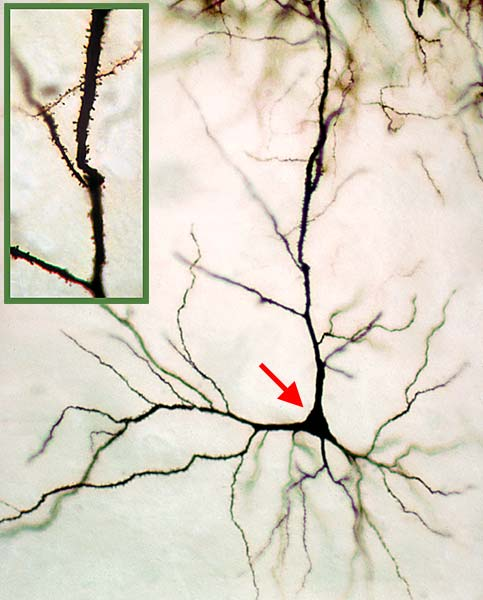
\includegraphics[width=0.7\textwidth]{Figures/Cochlear_nucleus_multipolar_cell.jpg}
 \caption[Pyramidal neuron]{A pyramidal neuron with an apical dendrite (staring by the arrow). The inset shows an amplification of the apical dendrite and illustrates the size of dendritic spines (small outgrowths). The arrow points to the cell body, called the Soma. Note that this image does not show how neurons are located within the brain. Image from \url{www.neurolex.org}.}
 \label{application:pyramidal_neuron}
\end{figure}

Figure \ref{application:pyramidal_neuron} shows a pyramidal neuron with an apical dendrite, and an inset with dendritic spines. 
Pyramidal neurons take their name from the triangular shape of the Soma, and an apical dendrite is a dendrite springing from the apex of the Soma. 
Spines are (often) the receiving end of a chemical synapse, which is a junction between two neurons that allows for communication between the two cells. \\

\noindent This application will look at diffusion of PKC$\gamma$ in an apical dendrite and into dendritic spines. 
PKC$\gamma$ is a protein found in neurons which is associated with memory storage and associative learning \cite{saito2002protein}. 
Upon activation it will diffuse out of the Soma, through a dendrite, and into a dendritic spine to reinforce or reduce the absorption of neurotransmitters. 
The results will be compared to results by Craske et.al \cite{craske2005spines}, who in 2005 studied a similar problem in rodent pyramidal neurons harvested from the hippocampus.

Effectively we will investigate the diffusion time for random walkers through spine necks which are very narrow ($\leq0.5\mu$m). Spine necks are thought to act as diffusion barriers which hinder, but do not stop diffusion \cite{craske2005spines}.

\section{Implementation}

There is a difference between the approach of the developed hybrid solver and the dendrite - spine system with respect to geometry which is best summarized in Figure \ref{application:geometry_difference}.\\

\noindent The dendrite is approximated as a cylinder with radius $\sim10\mu$m and length $\sim50\mu$m. Furthermore, little of interest is assumed to happen in the radial direction. All things considered, diffusion in the dendrite will be modeled as a 1D process. \\

\noindent Spines have a wide variety of geometries, with various properties. For this application, however, only the neck length and width of a spine is of interest. The spines will therefore be modeled as two dimensional objects with rectangular necks and trapezoidal heads. 
\begin{figure}[H]
 \centering
 \begin{subfigure}{0.48\textwidth}
  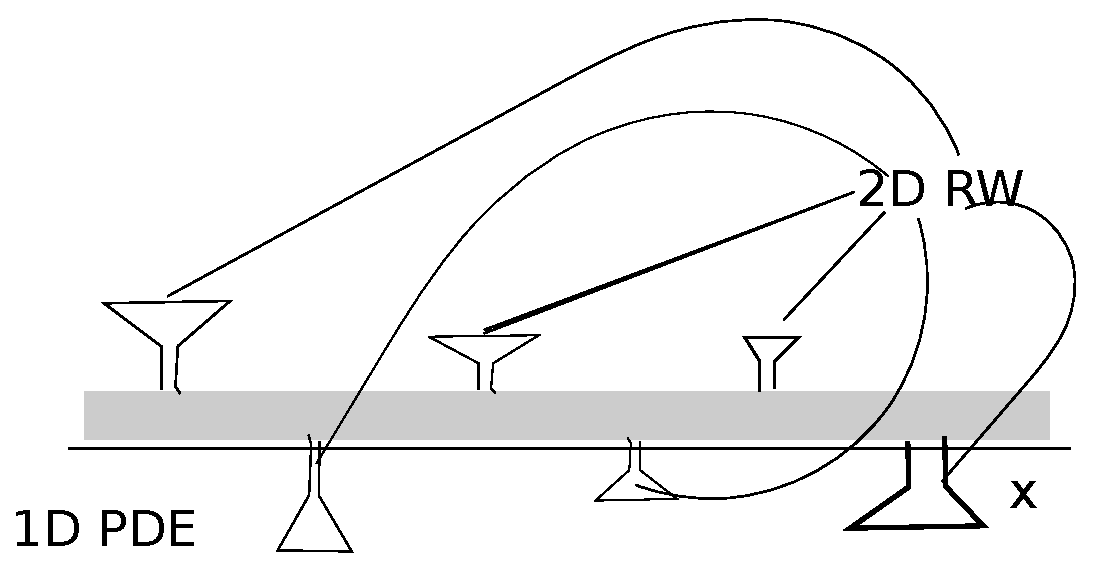
\includegraphics[width=\textwidth]{Figures/dendrite_spine_model.eps}
  \caption{}
 \end{subfigure}
 \begin{subfigure}{0.48\textwidth}
  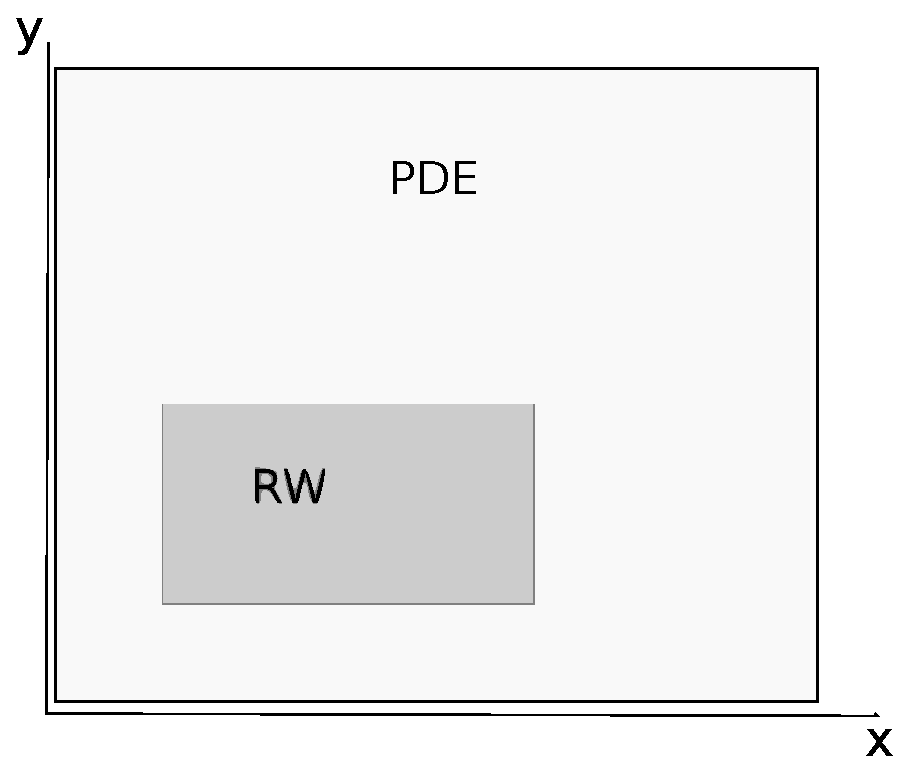
\includegraphics[width=\textwidth]{Figures/hybrid_model_principle.eps}
  \caption{}
 \end{subfigure}
 \caption[Difference between hybrid diffusion solver and dendrite - spine diffusion model]{The geometric difference between the original hybrid diffusion solver (b) and the numerical setup to model PKC$\gamma$ diffusing into dendritic spines (a). Spines are attached by a few mesh points on the PDE mesh, which also determines the neck width of the spine.}
 \label{application:geometry_difference}
\end{figure}

The hybrid diffusion solver has been slightly modified in order to recreate the new geometry. 
Mathematically the largest difference is that the random walkers are left alone, meaning that the diffusion equation is not solved in the spines. 
There are also some differences in the coupling; at each PDE time step there is a probability for an protein to diffuse into a spine if the concentration at the beginning of the spine neck is large enough. This probability decreases with the number of proteins which have already diffused into the spine. 
The width of a spine neck is determined by the number of PDE mesh points it connects to, which is chosen at random. 
All other length parameters are also determined randomly, but required to fit with measurements from Arellano et.al \cite{arellano2007ultrastructure}. 

\section{Parameters and details}
Within the first three seconds after PKC$\gamma$ is released from Soma, a portion of the released amount will bind to the Dendrite wall. 
This process is not governed by the diffusion equation, and seems to increase the speed with which PKC$\gamma$ diffuses into the spine \cite{craske2005spines}. 
For this application, these dynamics are not of interest. In order to still have a realistic model, the initial condition has been altered: 

Assuming that the actual release of PKC$\gamma$ from Soma can be modeled as a delta pulse, the solution will be a Gaussian function. 
The modified initial condition places a small amount of PKC$\gamma$ over the entire dendrite, and adds some random fluctuations. This is illustrated in Figure \ref{initial}. 
\begin{figure}[H]
 \centering
 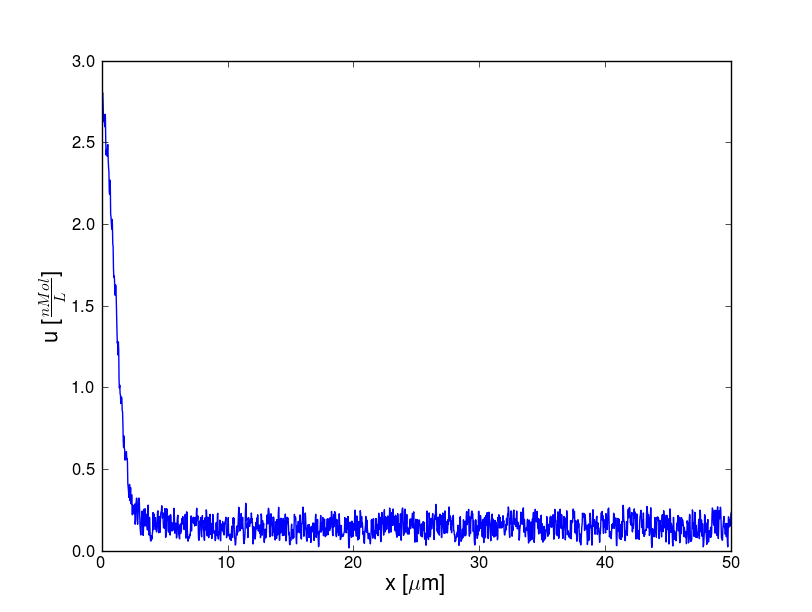
\includegraphics[width=0.6\textwidth]{Figures/initial_condition_application.png}
 \caption{Initial condition used in the application}
 \label{initial}
\end{figure}

\noindent The result of using this new initial condition is simply that approximately $3$ seconds can be added to all the measured times. \\

As Figure \ref{initial} shows, the concentration of PKC$\gamma$ has units $\frac{\text{nMol}}{\text{L}}$. 
Craske et.al. measured increases in concentration of around $5\frac{\text{nMol}}{\text{L}}$ in spine heads, which corresponds to $1-2$ proteins once the volume of a spine is taken into account. 
In fact, by calculating the volume of the dendrite segment we are simulating, the conversion factor has been estimated at $Hc = 5-25$. 

The model should have a few properties in order to be a realistic representation. First of all, if a large number of proteins are located at the junction to a spine, it is more likely that a protein diffuses into the spine. This is ensured by making the probability for a protein to diffuse into a spine to be dependent on the amount of PKC$\gamma$ present at the beginning of the spine neck. 

In order for a spine to be two dimensional, it must cover at least two points of the PDE mesh. This limits the minimal spatial resolution to the minimal neck diameter of a spine, which is $0.22\mu$m \cite{arellano2007ultrastructure}.

Real particles will ``feel'' a concentration gradient, but random walkers do not. As spine heads are filled with proteins, new proteins must therefore be hindered from entering a spine if it is full. 
